    \section{Von Neumannovy principy, blokové schéma Von Neumannova počítače. Rozdíl mezi Von Neumannovou, harvardskou a modifikovanou harvardskou architekturou. Procesory CISC a RISC. Rozdíl mezi obvodovým a mikroprogramovým řadičem. Řetězové zpracování instrukcí (pipelining), skokový a datový konflikt. Jak se liší a pro jaké typy úloh je určen mikroprocesor pro všeobecné použití, mikrokontrolér, signálový procesor a signálový kontrolér (DSC), SoC (System on a Chip), ASIC.}
\subsection{Von Neumnnova architektura}
\subsubsection*{Hlavní myšlenka}
Instrukce programu jsou reprezentovány binárními signály a jsou uloženy v paměti počítače spolu s daty. \\
\subsubsection*{Principy}
Principy:
\begin{itemize}
    \item Předpis pro řešení úlohy je převeden na posloupnost instrukcí
    \item instrukce a data se nacházejí ve stejné paměti
    \item Instrukce ani data nejsou explicitně označeny
    \item Paměť je rozdělena na stejně velká paměťová místa nazývaná adresy
    \item V instrukcích není uvedena hodnota operandu, ale jeho adresa
    \item instrukce se provádějí sekvenčně
    \item Toto sekvenční provádění lze narušit instrukcemi typu skok
\end{itemize}

\begin{figure}[h!]
    \centering
    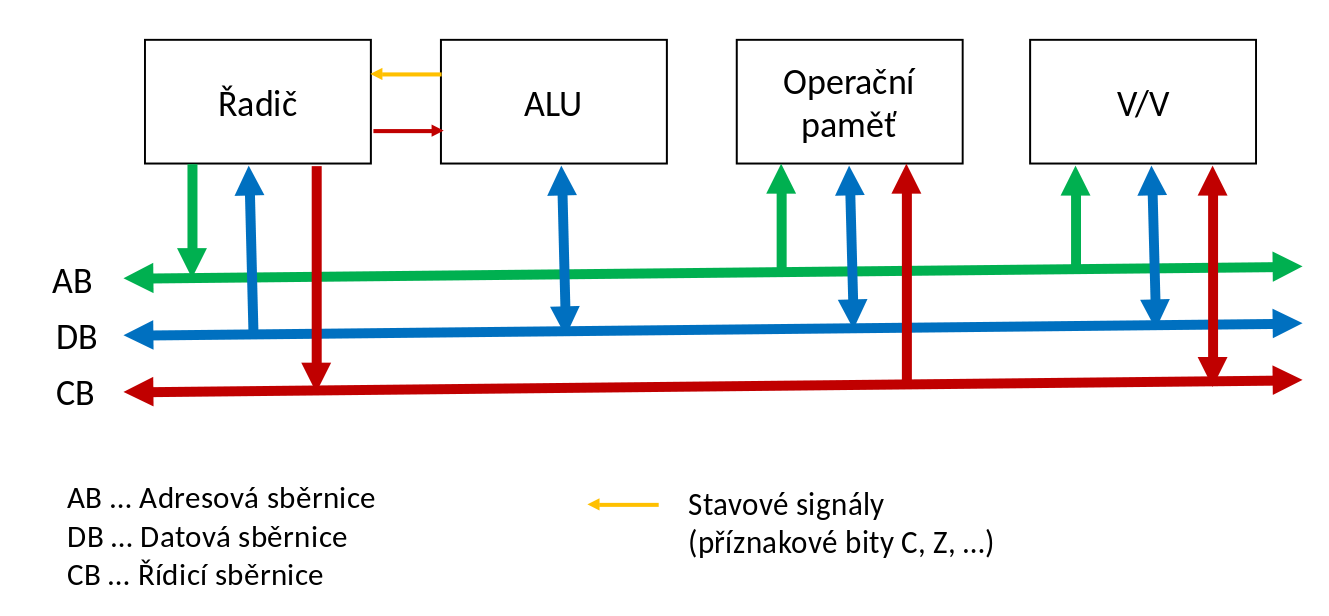
\includegraphics[width = \textwidth]{img/VonNeumann.png}
\end{figure}

\subsubsection*{Řadič}
Řídí činnost ostatních částí počítače. \\
Implementuje instrukční sadu. \\
Vstupy:\\
\begin{itemize}
    \item Signály z dekodéru instrukcí - dekóduje se část instrukce označována jako operační znak
    \item Signály generované ALU - Příznaky, přetečení, nulový výsledek, záporný výsledek
    \item Signál žádosti o obsluhu přerušení
\end{itemize}
Výstupy:\\
\begin{itemize}
    \item Čtení nebo zápis do paměti
    \item Čtení nebo zápis do periferie
    \item Signály ALU, určující kterou operaci má provést
\end{itemize}

\subsubsection*{ALU}
Aritmeticko-logická jednotka.\\
Provádí aritmetické operace(+,-,/,*), logické operace(AND,OR,NOT) a operace porovnání(>,<,=)\\
Řadič a ALU tvoří CPU. Integrací řadiče, ALU a registrů na jeden čip vzniká mikroprocesor.

\subsubsection*{Operační paměť}
Místo uložení dat a instrukcí.\\
Společná paměť pro instrukce a data. Jsou uloženy v jednom paměťovém prostoru.\\
U mikrokontrolerů jsou v instrukce v paměti FLASH a proměnné v paměti RAM, ale obě jsou připojeny ke stejným sběrnicím(AB,CB,DB)

\subsubsection*{V/V}
Slouží pro komunikaci s okolím.\\
Člověkem - klávesnice, myš, obrazovka. \\
Strojem, přístrojem či technologickým procesem - I/O, A/D, D/A převodníky a k nim akční členy - snímače. \\
S ostatními počítači a zařízeními pomocí sítě - Ethernet, WiFi moduly. \\
Umožňují ukládání dat na disky(SSD, HDD). \\

\subsubsection*{Registry}
Typy registrů:
\begin{itemize}
    \item Pracovní registr
          \begin{itemize}
              \item Ukládají operandy z ALU a výsledky z ALU
              \item Rychlejší než operační paměť
              \item Původně jeden registr nazývaný akumulátor
          \end{itemize}
    \item Stavový registr
          \begin{itemize}
              \item Skupina klopných obvodů ovládaných ALU
              \item Uchovávají stav ALU mezi instrukcemi
              \item Příznaky přetečení/výpůjčky, nulového či záporného výsledku
              \item Předcházející instrukce příznaky nastaví, následující využije
          \end{itemize}
    \item Programový čítač
          \begin{itemize}
              \item Zajišťuje sekvenční provádění instrukcí a provádění skoků
              \item V průběhu zpracování instrukce se nastaví tak aby obsahoval adresu následující instrukce
          \end{itemize}
\end{itemize}
Řídící a stavový registr bývají spojeny do jednoho řídícího stavového registru.\\

\subsubsection{Cyklus počítače}
Celý cyklus práce počítače se dělí na tyto opakující se části.
\begin{enumerate}
    \item Intruction fetch - načtení instrukce z paměti
    \item Intruction decode - dekódování instrukce
    \item Operand fetch - načtení operandu z registrů
    \item Intruction execution
    \item Write-back (Result store) - uložení výsledku
    \item Test, není-li požadavek na přerušení
\end{enumerate}
Nemusí se nutně vykonávat všechny tyto fáze.\\
Povinné fáze jsou pouze 1,2,4.

\subsection{Rozdíly mezi VonNeumannovou, harvardskou a modifikovanou harvardskou architekturou}
\subsubsection*{Von Neumannova architektura}
Společná paměť pro instrukce a data. \\
Existuje jedna datová a jedna adresová sběrnice. \\
Pomalejší oproti HA a MHA kvůli nutnosti číst instrukce nebo operand. \\
Výhoda spouštění programů z disků, jednoduchá změna počítače. \\
Dobře využitelná paměť. \\
Poloviční počet sběrnic oproti HA. Jednodušší konstrukce. \\
\begin{figure}[h!]
    \centering
    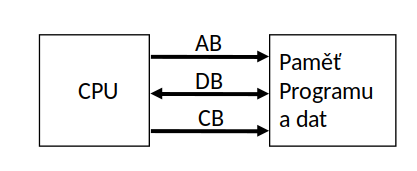
\includegraphics[]{img/VNporovnani.png}
\end{figure}

\subsubsection{Harvardská architektura}
Oddělena paměť dat a programu. To umožňuje číst obě zaráz a urychluje práci.\\
Může být různě adresována datová paměť a programová paměť.\\
Bezpečnější, nelze si poškodit program přepsáním jeho paměti.\\
Dvojnásobek sběrnic oproti VN, technologicky velký problém. \\
Nevyužitou část paměti nejde použít pro program a naopak. Z toho plyne, že je nižší efektivita využití paměti. \\
Využívá se u signálových procesorů, jinak moc ne.\\
\begin{figure}[h!]
    \centering
    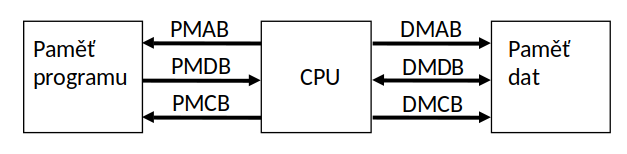
\includegraphics[width = \textwidth]{img/HAporovnani.png}
\end{figure}

\subsubsection*{Modifikovaná harvardská architektura}
Stejně jako HA 2 paměti. S rozdílem toho, že jedna je čistě pro data a druhá pro data a program.\\
Umožňuje číst 2 operandy zároveň díky rozmístění paměti. Toto umožňuje operaci Multiply and accumulate. \\
Využívá se u signálových procesorů a kontrolerů. \\

\begin{figure}[h!]
    \centering
    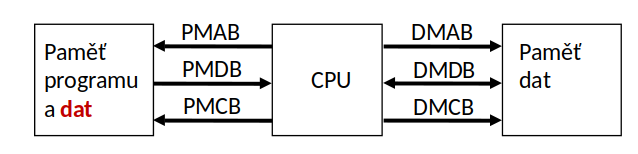
\includegraphics[width = \textwidth]{img/MHAporovnani.png}
\end{figure}

\subsection{Obvodový a mikroprogramový řadič}
\subsubsection*{Obvodový řadič}
Synchronní konečný stavový automat.\\
Logické členy a klopné obvody. \\
Umožňuje malou sadu jednoduchých instrukcí. \\
Výhodou je jednoduchost a malý počet součástek. \\
Nevýhodou je nutnost složité operace rozdělovat na více instrukcí. \\

\subsubsection*{Mikroprogramový řadič}
KSA, jehož kombinační část je tvořena pamětí mikroprogramu. \\
Implementuje složité instrukce za cenu složitosti řadiče. \\
Složité instrukce není možné přímo provést, proto jsou rozděleny na mikroinstrukce. \\
Posloupnost mikroinstrukcí, jimiž se vykoná instrukce se nazývá mikroprogram. \\
Mikroprogramy pro jednotlivé instrukce jsou uloženy v paměti mikroprogramu. \\
Toto zvyšuje složitost řadiče a počet cyklů potřebných na provedení instrukce. \\
Nutno operovat v nižších frekvencích kvůli problému s odvodem tepla. \\

\subsection{Procesory CISC a RISC}
\subsubsection*{CISC}
Complex instruction set computer. \\
Složité instrukční sady, přizpůsobené tak aby realizovaly příkazy programovacího jazyka. \\
Používá mikroprogramový řadič. \\
Stovky instrukcí. \\
Přesun složitosti z SW do HW. \\

\subsubsection*{RISC}
Reduced instruction set computer. \\
Malý počet jednoduchých instrukcí. \\
Vyšší nároky na překladače z programovacích jazyků. \\
Instrukce mají konstantní délku a jednotný formát, který vymezuje počet bitů v instrukci. \\
Obvodový řadič. \\
Velký počet registrů(16+), to snižuje nutnost častého přístupu do operační paměti. \\
Jediné instrukce, které mají povoleno interagovat s pamětí jsou \texttt{load} a \texttt{store}, load z paměti do registru, store naopak. Ostatní instrukce pracují pouze s registry.\\
V každém hodinovém taktu dokončena jedna instrukce. \\
Používá pipelining. \\

\subsubsection*{Post-RISC}
Kombinace CISC a RISC. \\
Rozšiřuje RISC o instrukce, které lze provádět rychle. \\
Hluboká pipeline až 10 kroků. \\
Více ALU pracujících paralelně. \\

\subsection{Řetězové zpracování instrukcí - pipelining}
Efektivnější využití času. \\
Každá fáze využívá jinou část CPU -> návrh procesoru pro paralelní práci na jeho částech. \\

\begin{figure}[h!]
    \centering
    \begin{minipage}[b]{0.4\textwidth}
        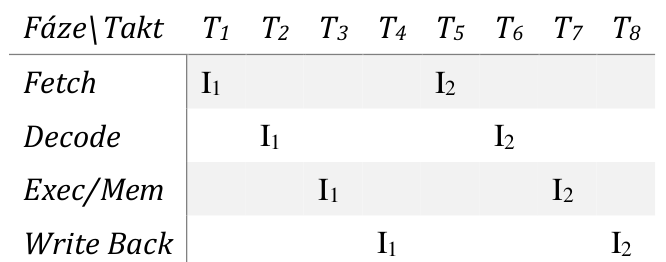
\includegraphics[width=\textwidth]{img/sekv.png}
    \end{minipage}
    \hfill
    \begin{minipage}[b]{0.4\textwidth}
        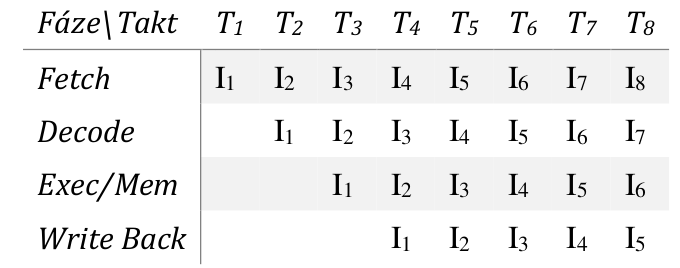
\includegraphics[width=\textwidth]{img/pipeline.png}
    \end{minipage}
\end{figure}

Doba exekuce instrukcí, kde k je počet fází:
\begin{center}
    Pipelining: \(N = k + (n-1)\) \\
    Sekvenční: \(M = n \cdot k\) \\
    Koeficient zrychlení: \(S_k = \frac{M}{N} = \frac{n \cdot k}{n + n-1}\)
\end{center}

\subsection{Skokový konflikt}
Při instrukci větvení nebo přerušení. Ve chvíli, kdy se začne provádět skok jsou v řetězci rozpracované instrukce. Řetězec tudíž musí být vyprázdněn a znovu naplněn, což vede ke snížení efektivity.\\
Řešení:
\begin{itemize}
    \item Predikce skoků
          \begin{itemize}
              \item Statická - nebere v úvahu historii provádění příslušné operace skoku. Například při provádění cyklu se skok provede vždy, instrukce obsahuje bit, který nastaví překladač (překladač odhaduje pravděpodobnost skoku)
              \item Dynamická - snaží se předpovědět skoky na základě chování programu v minulosti. Například provedl-li se skok při minulé exekuci dané instrukce počítá se, že se provede znovu. Procesor musí být vybaven spekulativní jednotkou
          \end{itemize}
    \item Použití dvou řetězců - 2 řetězce, jeden pro sekvenční provádění a druhý pro skoky.
\end{itemize}

\subsection{Datový konflikt}
Pokud instrukce pracuje s operandem z předchozí instrukce, která se však ještě nedokončila. \\

\begin{figure}[h!]
    \centering
    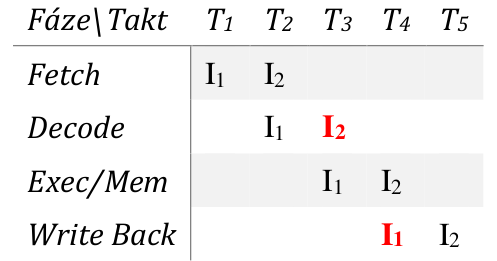
\includegraphics[scale = 0.4]{img/datKonf.png}
\end{figure}

Řešení:
\begin{itemize}
    \item Překladač řadí instrukce tak aby ke konfliktu nedošlo.
    \item Procesor detekuje konflikt a pozastaví konání $I_2$. Snižuje účinnost řetězení.
    \item Procesor detekuje konflikt a změní pořadí instrukcí. Náročné na konstrukci procesoru.
\end{itemize}

\subsection{Superpipelined procesor}
Procesor rozdělený na subprocesory, které zpracovávají instrukce jako řetězec. \\
Subprocesory je možné dělit na subbloky, které tvoří řetězce subprocesorů. \\

\subsection{Mikroprocesor, mikrokontrolér, signálový procesor, signálový kontroler,SOC, ASIC}
\subsubsection{Mikroprocesor pro všeobecné využití}
Na jednom čipu ALU, řadič, registry, případně cache a MMU.\\
Velký výpočetní výkon a paměťový prostor.\\
Stolní PC, notebooky, servery.\\
Modifikace pro telefony a tablety, optimalizovány na nízkou spotřebu, nižší výkon a paměť. \\

\subsubsection*{Mikrokontrolér}
Základní stavební kámen vestavných zařízeních. \\
Na jednom čipu procesor (řadič, ALU, registry, případně cache a MMU), paměti RAM a FLASH, řadič přerušení a periferie.\\
Menší výkon a paměť.\\
Určen pro embedded aplikace, spotřební elektronika, průmysl, automobily, řídící aplikace. \\

\subsubsection*{Signálový procesor - DSP}
Vznikly pro číslicové zpracování signálů v reálném čase a spektrální analýzu. \\
Vyžadují rychlé provádění specifických výpočetních operací, ale nepotřebují moc paměti. Například multiply and accumulate, v podstatě konvoluce, součin dvou parametrů a přičtení k proměnné.\\
Méně periferií než mikrokontrolery. \\
Dělí se na 2 typy:
\begin{itemize}
    \item S pevnou řádovou čárkou - jednodušší, levnější, algoritmy se hůře implementují
    \item S plovoucí řádovou čárkou, dražší, ale jednodušší implementace
\end{itemize}

\subsubsection*{Signálový kontroler - DSC}
Kombinace DSP a mikrokontroleru.\\
Má více periferií oproti DSP. \\
Využití pro výkonovou elektroniku. Měniče, vektorové řízení motorů.\\

\subsubsection*{System on a chip - SoC}
Integrovaný obvod, který zahrnuje všechny části počítače na jeden čip. \\
Digitální, analogové, rádiové, smíšené obvody na jednom čipu. \\

\subsubsection*{ASIC}
Integrovaný obvod navržený pro jednu aplikaci.\\
Většinou digitální, hromadná výroba.\\


\section{Rozdíl mezi izolovanými a paměťově mapovanými periferiemi. Způsoby obsluhy V/V: aktivní čekání, přerušení, DMA.
  Přerušení: řadič přerušení, činnost procesoru při zahájení obsluhy přerušení a návratu z přerušení, tabulka vektorů přerušení. Asynchronní a synchronní přerušení. Maskovatelné, nemaskovatelné a pseudomaskovatelné přerušení. Vnořené přerušení. RESET, činnost procesoru po RESETu.}
\subsection{Izolované a paměťově mapované periferie}
\subsubsection{Izolované}
Periferie využívají samostatný adresový prostor oddělený od adresového prostoru operační paměti.\\
Pro přístup k izolovaným periferiím se používají speciální instrukce.\\
Intel procesory mají společnou AB a DB pro periferie i operační paměť. instrukce IN a OUT.

\subsubsection*{Paměťově mapované}
Periferie se nacházejí ve stejném paměťovém prostoru jako operační paměť. \\
Pro přístup k periferiím se používají stejné instrukce jako pro přístup k operandům v operační paměti.\\
\subsection{Způsob obsluhy V/V}
\subsubsection*{Řídící registry periferií}
Různé periferie se značně liší, ale práce s nimi je do jisté míry podobná.\\
Z hlediska programátora jsou důležité registry periferií, které se podle funkce dají rozdělit:
\begin{itemize}
    \item Konfigurační (řídící) registry - slouží pro nastavení režimu fungování periferie.
    \item Stavové (příznakové) registry - obsahují příznakové bity (flagy), které signalizují stav periferie (např. stavový registr A/D převodníku obsahuje bit signalizující dokončení převodu)
    \item Datové registry - slouží pro vyčítání nebo ukládání dat, které periferie zpracovává
\end{itemize}

\subsubsection*{Obsluha pomocí aktivního čekání - busy waiting, pooling}
Procesor odstartuje V/V operaci zápisem do řídícího nebo datového registru a pak ve smyčce testuje, zda-li byla operace dokončena nebo došlo k chybě - to značí příslušný bit (flag).\\
Velká nevýhoda je, že během čekání ve smyčce procesor nemůže provádět jinou užitečnou činnost => plýtvání času.\\
V embedded systémech hrozí, že dojde k promeškání důležité události (např. nárust tlaku v nádobě => havárie).\\
Jediná výhoda je jednoduchá implementace, využívá se při testování u vývoje periferií.\\

\subsubsection*{Obsluha pomocí přerušení}
Procesor odstartuje V/V operaci zápisem do řídícího nebo datového registru. \\
Nečeká na dokončení operace, ale provádí jinou užitečnou činnost.\\
Po dokončení operace nebo při chybě periferie generuje požadavek na přerušení.\\
Procesor rozpozná požadavek na přerušení a dočasně přeruší provádění aktuálního kódu a vykoná kód obslužné rutiny přerušení pro danou periferii. \\
Po vykonání obslužné rutiny se procesor opět vrátí k vykonávání kódu, který prováděl před přechodem do přerušovací rutiny.\\

\subsubsection*{Obsluha pomocí DMA}
Některé periferie (např. řadiče disků) obsahují vyrovnávací paměti.\\
Při provádění V/V operací je třeba přenášet větší množství bytů mezi operační pamětí a vyrovnávací pamětí periferie. \\
Je výhodné, aby přenos dat probíhal bez účasti procesoru a procesor mohl provádět jinou užitečnou činnost. Aby toto bylo možné musí v počítači být řadič sběrnic - DMA. Během přenosu dat CPU uvolní sběrnice a ty převezme řadič DMA. DMA generuje adresy a řídící signály jako MEMR a MEMW.
Před zahájením DMA přenosu musí procesor na DMA nakonfigurovat:
\begin{itemize}
    \item Počáteční adresu v operační paměti.
    \item Počáteční adresu v paměti periferie.
    \item Směr přenosu.
    \item Počet přenášených bytů.
\end{itemize}

\subsection{Přerušení}
\subsubsection*{Použití přerušení}
Používá se pro obsluhu neodkladných událostí. \\
Při požadavku na přerušení procesor přeruší aktuálně prováděný kód a provede kód obsluhující událost a vrátí se zpět.\\
Kód obsluhy se nazývá obslužná rutina přerušení.\\
Používá se pro obsluhu periferií, nebo k ošetření výjimečných situací jako chyby a havarijní stavy (např. dělení nulou, chyba ochrany paměti, pokles napájecího napětí atd.).\\
Přerušení lze také vyvolat softwarově pomocí příslušné instrukce. Používá se pro přístup ke službám jádra operačního systému. Na některých procesorech je to jediný způsob, jak lze přejít z uživatelského módu na mód supervisor (v němž běží jádro operačního systému)

\subsubsection*{Řadič přerušení}
Počítač obvykle používá více V/V periferií, které mohou generovat požadavky na přerušení.\\
Jednotlivé zdroje přerušení jsou připojeny na vstupy bloku počítače nazývaného řadič přerušení.\\
Aby procesor mohl určit zdroj přerušení, je ke každému zdroji přiřazeno celé kladné číslo. Periferie nastaví aktivní úroveň signálu na vstup řadiče a ten zašle číslo přerušení. Periferie mají z hlediska obsluhy různou prioritu, podle toho se řadič rozhoduje, co oznámí procesoru jako první, když je současně generováno víc požadavků.\\
Priorita buď softwarově nebo hardwarově, softwarovou můžeme měnit zápisem do řadiče.\\
Dnešní počítače vybavené sběrnicí PCI Express nepoužívají dedikované vodiče pro komunikaci mezi řadičem a procesorem, periferie posílají požadavek na obsluhu jako zprávu po sběrnici PCIe. Zpráva je posílána na speciální adresu v paměťovém prostoru. Tento způsob přerušení se nazývá MSI ( Message Signaled Interrupts).

\subsubsection*{Činnost procesoru při obsluze přerušení}
Při příchodu požadavku na asynchronní nebo softwarové přerušení procesor dokončí prováděnou instrukci. \\
Na konci instrukčního cyklu procesor testuje, jestli není požadavek na obsluhu přerušení, pokud je, tak procesor zahájí obsluhu:
\begin{enumerate}
    \item Uloží do zásobníku návratovou adresu
    \item Uloží do zásobníku obsah stavového registru
    \item Některé procesory ukládají do zásobníku obsah pracovních registrů
    \item V příznakovém registru nastaví bit I, čímž zakáže přerušení. Během provádění obslužné rutiny jsou maskovatelná přerušení zakázána, pokud je programátor v přerušovací rutině explicitně nepovolí
    \item Procesor na základě čísla přerušení stanoví adresu vektoru přerušení. Na adrese vektoru přerušení se musí nacházet adresa první instrukce obslužné rutiny
    \item Procesor vyzvedne adresu první instrukce z vektoru přerušení a vloží ji do programového čítače - tím se začne provádět obslužná rutina
\end{enumerate}
Poslední instrukce obslužné rutiny přerušení musí být instrukce návratu z přerušení (RTI), která zajistí, že procesor:
\begin{itemize}
    \item Pokud procesor uložil obsah pracovních registrů, obnoví jejich obsah
    \item Obnoví ze zásobníku obsah stavového registru - tím se povolí maskovatelná přerušení (nastavení bitu I)
    \item Vyzvedne ze zásobníku návratovou adresu a vloží ji do programového čítače, v případě asynchronního přerušení procesor pokračuje následující instrukcí, u výjimek (např. dělení nulou) se restartuje instrukce, která výjimku způsobila
\end{itemize}
Pokud má procesor větší množství pracovních registrů, ukládání pracovních by trvalo nepřijatelně dlouho, přitom by programátor nebo překladač obsah některých registrů v přerušovací rutině nemodifikoval. Proto procesory s větším množství registrů tyto registry automaticky neukládají a je odpovědnost programátora nebo překladače uložit ty registry, které se budou modifikovat.\\
Existují procesory, které mají pracovní registry zdvojené a jen se přepíná mezi hlavními a stínovými(pro rutinu) registry. Přepínání je rychlé, ale velmi náročné na konstrukci. Toto řešení je dnes spíše výjimkou. \\

\subsubsection*{Vektor přerušení}
Adresa kde se nachází první instrukce obslužné rutiny.\\
Každý zdroj přerušení má svůj vektor přerušení.\\

\subsubsection*{Tabulka vektorů přerušení}
Oblast paměti kde jsou za sebou umístěny vektory přerušení.\\
Číslo vektoru je indexem tabulky vektorů.\\
Řadič předá procesoru číslo vektoru přerušení, procesor vynásobí číslo vektoru přerušení velikostí vektoru přerušení a výsledek přičte k adrese začátku tabulky vektorů přerušení.\\
Počáteční adresa tabulky bývá u jednoduchých procesorů daná výrobcem napevno, složitější na to mají speciální registr, kde se napíše námi zvolená adresa.

\subsubsection*{Asynchronní a synchronní přerušení}
\begin{itemize}
    \item Asynchronní
          \begin{itemize}
              \item nejsou synchronizovány s prováděním instrukcí v CPU
              \item jsou vyvolány asynchronními událostmi
              \item typické zdroje jsou V/V periferie - dokončení AD převodu, doběhnutí časovače, příjem ethernet rámce, zmáčknutí klávesy, detekce poklesu napětí
          \end{itemize}
    \item Synchronní
          \begin{itemize}
              \item Generována v důsledku provádění určitých instrukcí v přesně definované fázi zpracování dané instrukce.
              \item Přerušní generují instrukce softwarového přerušení a výjimky
              \item Výjimky jsou generovány kontrolními obvody počítače, když dojde k chybě v provádění instrukce. Typické výjimky jsou dělení nulou, pokus o exekuci neznámé či ilegální instrukce, neoprávněný pokud o přístup k paměti
          \end{itemize}
\end{itemize}

\subsubsection*{Maskovatelná přerušení}
Přerušení lze povolit nebo zakázat obvykle nastavením (vynulováním) bitu I v příznakovém registru.\\
Např. Program provádí úsek kódu kde pracuje s proměnnými, které používá přerušovací rutina, před začátkem práce s těmito proměnnýma zakáže přerušení a provede manipulaci a pak opět povolí přerušení.\\

\subsubsection*{Nemaskovatelná přerušení}
Kritické události jako porušení paměti nebo výpadek napájení je však třeba obsloužit vždy. \\
Tyto přerušení musí být povolena vždy a nesmí být možnost je zakázat.\\
Například porušení paměti či výpadek napájení. \\

\subsubsection*{Pseudomaskovatelná přerušení}
U nemaskovatelných vznikal problém při zahájení činnosti procesoru po RESETu. Obsluha přerušení vyžaduje minimálně nastavení ukazatele zásobníku na adresu začátku zásobníku  v paměti RAM. Vyvolání přerušení v okamžiku, kdy není nastaven ukazatel může způsobit zhroucení celého systému. Proto je potřeba po dobu základní inicializace zabránit obsluze jakýchkoliv přerušení, tedy i nemaskovatelných. \\
Toto přerušení je po resetu zakázáno, ale po inicializaci systému se přerušení povolí a do dalšího resetu jej nejde zakázat a chová se jako nemaskovatelné. \\

\subsubsection*{Vnořená přerušení}
Může nastat situace, kdy procesor provádí obslužnou rutinu přerušení a během ní dojde požadavek na další přerušení. \\
Pokud mají stejnou prioritu, tak se první provede jedna a pak až druhá obsluha.\\
V praxi to tak ale většinou není, většinou jedno přerušení má větší prioritu. Takže uprostřed prvního přerušení se provede druhé přerušení (vnořené) a po vykonání se vrátí k prvnímu a to se dokončí.\\
\subsection{RESET a činnost procesoru po RESETu}
RESET procesoru způsobí nastavení procesoru do definovaného výchozího stavu.\\
Z hlediska uživatele to znamená, že se vynulují pracovní registry a řídící registry se nastaví na výrobcem definované hodnoty.\\
Po uvolnění signálu RESET procesor vyzvedne z definované adresy reset vektor adresu první instrukce a vloží ji do programového čítače.\\
Adresa reset vektoru je definována výrobcem a musí být v pevné paměti.\\
Stejně tak musí být první instrukce uložena v pevné paměti. Dnes uloženy ve FLASH paměti kde je UEFI, které provádí inicializaci V/V periferií a zavedení OS.\\
U jednoduchých kontrolerů bývá reset poslední vektor v tabulce přerušení.\\

\section{Princip a vlastnosti pamětí ROM, EEPROM, FLASH. Rozdíl mezi paměťmi NOR FLASH a NAND FLASH. Princip pamětí MRAM a FeRAM.}
\subsection{ROM}
Obsah paměti naprogramován při výrobě a nelze změnit. \\
Pro velké objemy výroby. \\
Buňka tvořena tranzistorem MOSFET zapojeným mezi sloupec a zem. \\
Hradlo tranzistoru je připojeno k řádkovému vodiči. \\
U funkčních tranzistorů je mezi hradlem a polovodičem vyleptána tenká vrstva oxidu křemíku. U nefunkčních je vrstva tlustá. \\
Po vybuzení řádkového vodiče dojde u funkčních tranzistorů k vytvoření indukovaného kanálu a tím ke zkratování sloupce na zem (Úroveň Low - logická 0). U nefunkčních kanál nevznikne, tranzistor je nevodivý a sloupec zůstává na úrovni High - logická 1. \\
Proleptání se dělá pomocí masky, kterou se určí který tranzistor bude 0 a který 1. \\

\subsubsection*{PROM}
Obsah paměti si uživatel jednorázově naprogramuje sám. \\
Pak paměť již nelze měnit. \\

\subsubsection*{Tranzistor s plovoucím hradlem}
Pokud jsou ve floating gate elektrony tak se zvyšuje potřebný potenciál na aktivaci tranzistoru a tudíž se tranzistor neaktivuje a představuje logickou 0. \\
Pokud v ní nejsou elektrony, tranzistor se zaktivuje a tudíž představuje logickou 1. \\
Programování a mazání:
\begin{itemize}
    \item Tunelování elektronů
          \begin{itemize}
              \item Programování: Na source a control gate se přivede zvýšené napětí, na source záporný pól a na CG kladný. Tím jsou elektrony tunelovány skrze tenkou vrstvu izolantu do floating gate a tranzistor je naprogramován na logickou 0
              \item Mazání: Na control gate je přiveden záporný pól a na source kladný, tím se tranzistor vybije a změní se na logickou 1.
          \end{itemize}
    \item Lavinová injekce
          \begin{itemize}
              \item Programování: Mezi source a drain se vyvolá velký proud přivedením napětí, elektrony získají velkou energii a mohou opustit kanál. Na control gate se přivede zvýšené napětí, které tahá elektrony z kanálu a ty uvíznou ve floating gate.
              \item Vybíjení: Nelze
          \end{itemize}
\end{itemize}

\begin{figure}[h!]
    \centering
    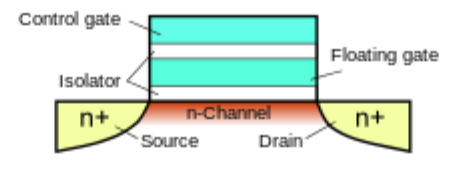
\includegraphics[]{img/FGMOS.png}
\end{figure}
\subsubsection*{EPROM}
Paměťová buňka obsahuje jeden paměťový tranzistor FAMOS (floating Gate Avalanche Injection MOS) - neboli tranzistor s plovoucím hradlem asi. \\
Obsah paměti si uživatel naprogramuje sám, je programovatelná elektricky pomocí zvýšeného napětí. \\
Lze mazat UV zářením. \\
Před programováním musí být paměť vymazána. \\
Počet cyklů programování - mazání je cca desítky. \\

\subsubsection*{EEPROM}
Paměťová buňka složena ze 2 tranzistorů. Paměťový tranzistor s plovoucím hradlem. Výběrový tranzistor je MOS, je potřeba abychom mohli měnit obsah každé buňky nezávisle na ostatních. \\
Obsah paměti lze programovat a mazat pomocí elektrických
signálů bez předchozího vymazání. \\
Narozdíl od RAM trvá zápis o několik řádů delší dobu než čtení.     Čtení i zápis v RAM trvá cca nanosekundy, stejně jako čtení paměťového místa EEPROM, zápis ale trvá cca milisekundy. \\
K zápisu i mazání využívá tunelování elektronů. \\
\begin{figure}[h!]
    \centering
    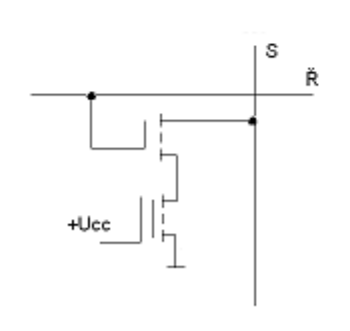
\includegraphics[scale = 0.5]{img/EEPROM.png}
\end{figure}

\subsubsection*{FLASH}
Paměťová buňka tvořena pouze jedním tranzistorem.\\
Speciální druh paměti EEPROM, který umožňuje mazat či zapisovat na více paměťových míst pomocí jedné programovací operace - mazána může být např. celá paměť nebo jen zvolená oblast paměti najednou. \\
Elektricky programovatelná za pomocí lavinové injekce(rychlé), mazání za pomoci tunelování elektronů(pomalé).\\
Mechanismus ochrany proti zápisu - možnost dočasně udělat z paměti read-only. Zápis se pak povolí zapsáním definované sekvence bytů do řídících registrů paměti.\\
Vyšší hustota oproti EEPROM. \\

\subsubsection*{NOR FLASH}
Každý tranzistor je zapojen paralelně ke sloupcovému vodiči. Umožňuje samostatně adresovat každou paměťovou buňku.\\
Programování pomocí lavinové injekce, mazání tunelováním. \\
Rychlé čtení dat s náhodným přístupem. Možnost čtení i zápisu po bytech.\\
Oproti NAND FLASH pomalý zápis a mazání. Pro aplikace kde se data moc nemění.\\
Přímá náhrada ROM, EEPROM, stejné připojení k procesoru.\\
Používá se pro ukládání firmware v embedded systémech a pro ukládání kódu zavaděčů OS(BIOS/UEFI).\\
Každý tranzistor přivedeme mezi zem(source) a sloupcový vodič(bit-line).\\
Stačí jeden sepnutý tranzistor aby se bit-line stáhnul do nízké hodnoty. \\

\subsubsection*{NAND FLASH}
Několik paměťových buněk zapojeno do série. Každý paměťový tranzistor nemusí být připojen ke sloupcovému
a zemnímu vodiči -> menší paměťová buňka (hustota informace
až o 45\% vyšší než NOR FLASH).\\
Pro programování i mazání se používá tunelování elektronů.\\
Složitější rozhraní než paměti NOR FLASH. Nelze je přímo připojit ke sběrnicím mikroprocesoru. Čtení s náhodným přístupem je pomalé, proto není možné z paměti přímo provádět kód. \\
Čtení: na všechny tranzistory ve skupině mimo čteného se přivede vyšší než prahové napětí(všechny se sepnou). Na čtený se přivede napětí vyšší jak práh pro vybitý tranzistor, ale nižší než pro nabitý. Pokud je vymazán sepne se a bit line stáhne do 0, pokud není vymazán bit line zůstane na vysoké úrovni. \\
Nevýhoda je přítomnost vadných bitů, které časem přibývají.\\
Vhodné pro aplikace kde je potřeba ukládat velké množství dat, používá se sekvenční čtení, není potřeba provádět kód přímo z FLASH.\\
USB a SSD disky.\\

\begin{figure}[h!]
    \centering
    \begin{minipage}[b]{0.4\textwidth}
        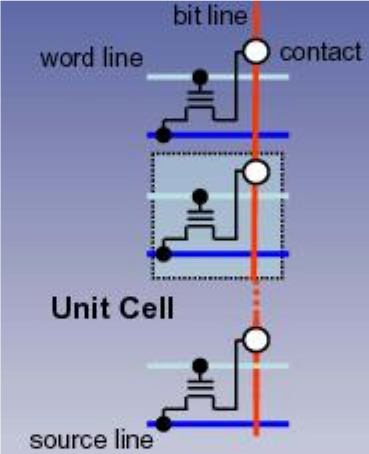
\includegraphics[width=\textwidth]{img/NOR.png}
    \end{minipage}
    \hfill
    \begin{minipage}[b]{0.4\textwidth}
        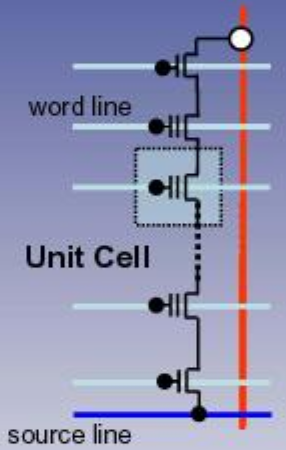
\includegraphics[width=\textwidth]{img/NAND.png}
    \end{minipage}
    \caption*{Nalevo NOR, napravo NAND}
\end{figure}


\subsubsection*{FeRAM}
Konstrukčně obdobné DRAM paměti, ale dielektrikum je tvořeno feroelektrickým materiálem.\\
Informace je zachována i po vypnutí napájení.\\
Uplatnění v průmyslových a bankovních systémech.\\
Výhody oproti FLASH - vyšší počet cyklů mazání(\(10^{16}\)), vyšší rychlost zápisu, nižší spotřeba.\\
Nevýhody oproti FLASH - malá hustota, limitovaná max kapacita, vyšší cena.
Základem jsou feroelektrické krystaly. Založeno na vystavení feroelektrického krystalu elektrickému poli, centrální atom v mřížce krystalu se vychýlí ve směru elektrického pole. a zapříčiní proudový náraz. Ten je zaznamenán vnitřními obvody a paměť je následně zapnuta. Díky tomu, že atom zůstane vychýlen i po odstranění pole zůstává informace uchována.
Feroelektrický materiál uvnitř feroelektrického kondenzátoru v podobě tenkého filmu mezi elektrodami.
\begin{figure} [h!]
    \centering
    \includegraphics*[scale = 0.3]{img/FeRAM.png}
\end{figure}

\subsubsection*{MRAM - Magnetoresistive RAM}
Uplatnění v ukládání dat v uzlech IoT, aplikace strojového učení a umělé inteligenci.\\
Magnetorezistivní jev, změna odporu materiálu vlivem působení magnetického pole. Odpor se mění podle orientace magnetického pole při zápisu bitu.\\
V MRAM se používá tunelová magnetorezistence - TMR. změn R o 30-70\%.\\
TMR nastává na přechodu mezi dvěma feromagnetickými plátky oddělenými tenkým izolátorem. Dielektrická vrstva oxidu hliníku.\\
Každý plátek může být zmagnetizován. \\
Jeden plátek tvoří permanentní magnet s neměnnou orientací magnetického pole.\\
Magnetizace druhého plátku je nastavována vnějším polem tak, aby orientace jeho pole odpovídala zapamatování 1 nebo 0.\\
Paralelní magnetizace je logická 0, antiparalelní magnetizace logická 1.

\begin{figure}[h!]
    \centering
    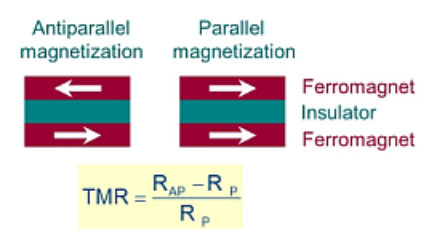
\includegraphics[scale = 0.5]{img/MRAM.png}
\end{figure}

Rychlost srovnatelná s SRAM. Hustota informace jako DRAM. Rychlejší než FLASH, menší spotřeba než DRAM.

Princip: Pokud je směr magnetického pole proměnné feromagnetické vrstvy (plátku) stejný s pevně daným směrem spodní vrstvy, je odpor kladený elektrickému proudu malý. Pokud je vzájemná orientace polí opačná, je vertikální elektrický odpor struktury velký. Změna logického stavu z 0 na 1 nebo z 1 na 0 se provádí přivedením sekvence dvou vzájemně posunutých proudových obdélníkových pulsů na dva zápisové vodiče paměťové buňky.\\
Čtení stavu bitu se provádí prostřednictvím jedné společné elektrody a menší speciální čtecí elektrody napojené na protější stranu vertikální struktury.\\
Zapsaný stav 1 - buňka má větší odpor a naopak.\\

\section{Princip a vlastnosti statických pamětí RAM (SRAM) a synchronních dynamických paměti DRAM (SDRAM).
  Připojování paralelních pamětí SRAM, FLASH ke sběrnicím mikroprocesoru. Adresový dekodér.
  Hierarchie paměti, paměti cache, specializované paměti cache.}

\subsection{SRAM a SDRAM}
\subsubsection*{SRAM - Statická RAM}
Paměťová buňka tvořena bistabilním klopným obvodem.\\
Paměťová buňka je rychlá, ale velká – tvořena 6 tranzistory.\\
Využívá se jako procesorová Cache.\\
Výhodou je vysoká rychlost čtení a zápisu. Nevýhodou malá hustota oproti DRAM.\\
Snadné připojení k CPU.\\
\begin{figure}[h!]
    \centering
    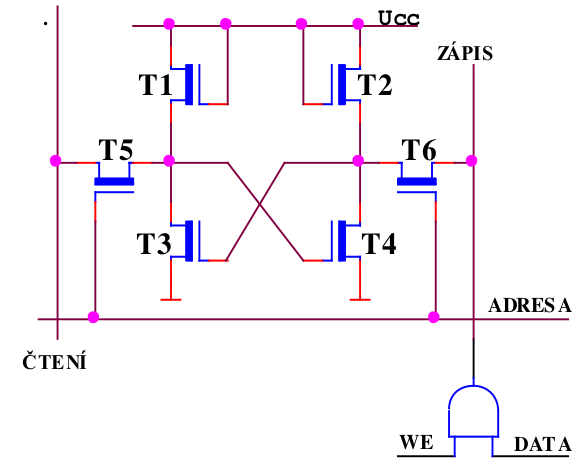
\includegraphics[scale = 0.3]{img/SRAM.png}
\end{figure}

\subsubsection*{SDRAM}
Zavedení synchronizačních (hodinových) impulsů.\\
Všechny vstupní signály jsou náběžnou hranou hodinového impulsu
zapsány do vnitřních registrů.\\
Vnitřní signály se tak mění v přesně definovaných okamžicích a naopak na časování vnějších signálů jsou kladeny podstatně menší nároky než u jednoduché DRAM.\\
Lze na ně zapisovat shluky dat(bytů) - burst reading/writing. Velikosti 1,2,4,8,16B(DDR5) velikost shluku obvykle odpovídá velikosti cache.
Obsahují několik paměťových matic nazývaných banky. Jednotlivé banky mohou pracovat samostatně. Banky jsou dále děleny na řádky(stránky, pages). Dále jsou řádky děleny na sloupce, v každém řádku 1Ki sloupců.\\
Adresa je tvořena:
\begin{itemize}
    \item Adresou skupiny bank: BG0-BG1
    \item Adresou banky: BA0-BA1
    \item Adresou řádku: A0-A14
    \item Adresou sloupce
\end{itemize}

\subsection{Připojování paralelních pamětí SRAM, FLASH ke sběrnicím procesoru}
\begin{itemize}
    \item \(A_x\) - adresové sběrnice
    \item \(D_x\) - datové sběrnice
    \item MEMR\ - řidicí sběrnice memory read
    \item MEMW\ - řidicí sběrnice memory write
    \item OE\ - output enable
    \item WE\ - write enable
    \item CS\ - chip select - slouží pro výběr paměťového čipu
\end{itemize}
\begin{figure}[h!]
    \centering
    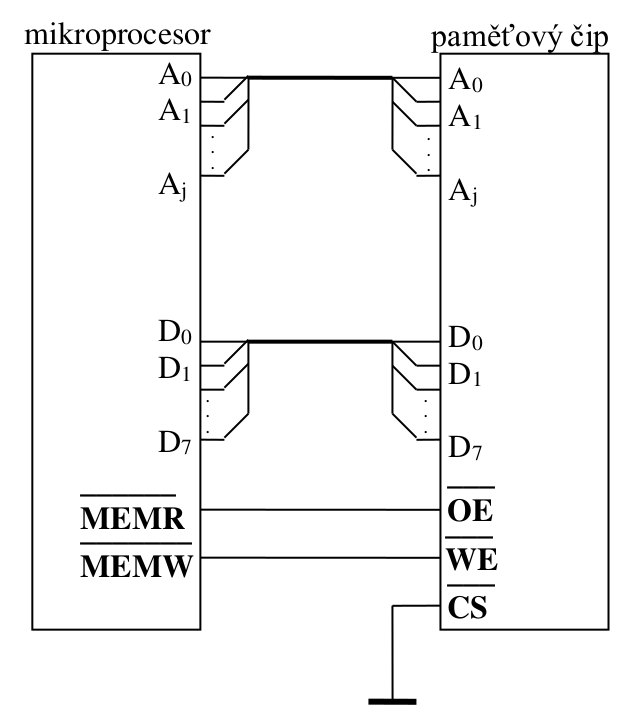
\includegraphics[scale = 0.3]{img/MemConnect.png}
\end{figure}

\subsubsection*{Adresový dekodér}
Binární dekodér zajišťuje rozdělení
paměťového prostoru na jednotlivé čipy.\\
Na základě nejvyšších bitů adresy je aktivován vždy pouze jeden výstup adresového dekodéru, který aktivuje příslušný čip.\\

\begin{figure}[h!]
    \centering
    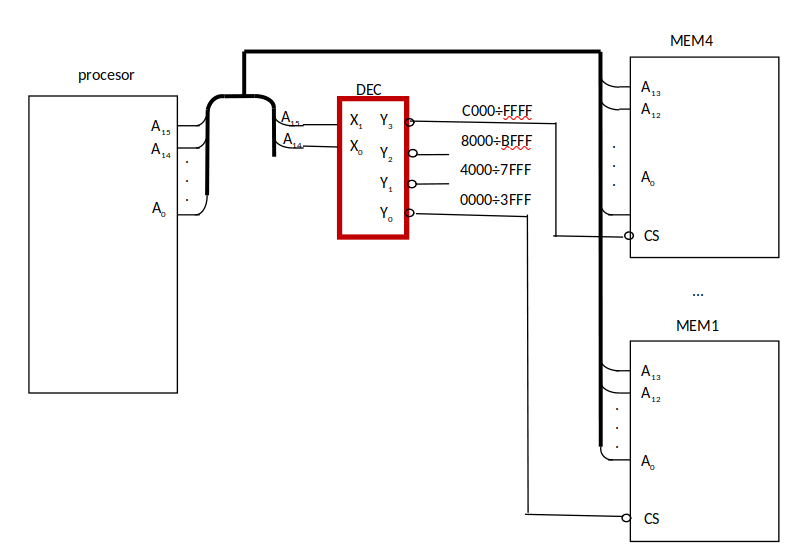
\includegraphics[scale = 0.35]{img/AdrDekoder.png}
\end{figure}
\newpage
\begin{figure}
    \centering
    \includegraphics*[width = \textwidth]{img/AdrDekTab.png}
\end{figure}

\subsection{Hierarchie paměti, paměti cache a specializované cache}
Procesory jsou o několik řádů rychlejší než operační paměť, tudíž musí čekat, což je plýtvání časem.
Chování programů jde popsat pomocí lokalit instrukcí a dat.
\subsubsection*{Časová lokalita instrukcí}
Je-li použita instrukce, dá se očekávat, že se brzy použije znovu.
\subsubsection*{Prostorová lokalita instrukcí}
Je-li použita instrukce, dá se očekávat, že se brzy použije instrukce na blízké adrese.

\subsubsection*{Hierarchie paměti}
Schéma VonNeumannova počítače je doplněno o vyrovnávací paměti procesoru takzvané cache, které jsou umístěny mezi procesor a hlavní paměť.
\begin{figure}[h!]
    \centering
    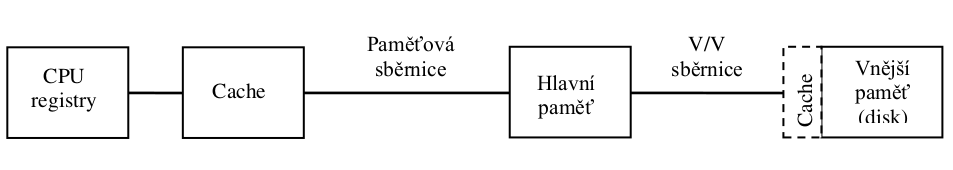
\includegraphics[width = \textwidth]{img/Hierarchie.png}
\end{figure}
Hierarchií rozumíme několik úrovní pamětí různých kapacit a rychlostí. Jsou seřazeny dle kapacity vzestupně a rychlosti sestupně.
\begin{enumerate}
    \item Registry - nejblíže procesoru, stejně rychlé jak procesor, avšak s velmi malou kapacitou
    \item Cache - kapacitně jednotky až nižší desítky MB, ale rychlá a drahá SRAM paměť
    \item Hlavní operační paměť
    \item Vnější disk - nejvyšší kapacita, avšak velmi pomalé
\end{enumerate}
\subsubsection*{Cache}
Mezi procesorem a hlavní pamětí. \\
Obsahuje často používané instrukce a data, aby nebylo nutné je číst z hlavní paměti. \\
Když procesor potřebuje číst nebo zapisovat do hlavní paměti, prve se podívá zda tu data jsou, pokud ano pro čtení a ne pro psaní tak data zapíše do cache což je mnohem rychlejší než psaní nebo čtení do/z hlavní paměti. \\
Cache hit - procesor našel v cache, Cache miss - nenašel, hit rate - úspěšnost hitů.\\
Menší cache je rychlejší, ale čím větší je tím má větší hit rate.\\
Dělí se na 3 typy
\begin{itemize}
    \item L1 - nejmenší a nerychlejší, pro každé jádro zvlášť, při přístupu nemusí procesor čekat.
    \item L2 - větší, pomalejší, pro každé jádro zvlášť, při přístupu čeká 1 až 2 hodiné takty.
    \item L3 - největší, společná pro všechny jádra.
\end{itemize}

\subsubsection*{Specializované cache}
Většina moderních procesorů má alespoň 3 nezávislé cache.\\
\begin{itemize}
    \item Instruction cache - pro instrukce
    \item Data cache - pro data procesoru
    \item TLB cache - Translation look-aside buffer cache, zrychluje překlad fyzických adres na fyzické
\end{itemize}

\section{Zdroje hodinových impulsů pro mikrokontroléry, jejich parametry. Fázový závěs (blokové schéma, funkce, důvody použití). Princip a použití watch dog. Komunikační rozhraní UART, SPI a IIC.}

\subsection{Zdroje hodinových impulsů pro mikrokontroléry}
Každý synchronní sekvenční logický obvod potřebuje být taktován hodinovými impulsy. Hodinové impulsy potřebuje pro svoji činnost jádro (CPU) i periferie. PC, notebooky, servery mají na základní desce krystalový oscilátor, procesor je buzen impulsy z tohoto externího oscilátoru. 
Mezi zdroje hodinovývh impulsů žadíme:
\begin{itemize}
    \item Externí zdroje: Obvykle krystalový oscilátor umístěný vně čipu.
    \item Znitřní zdroje: 
    \begin{itemize}
        \item Vnitřní RC oscilátor (méně přesný, ale nevyžaduje externí součástky).
        \item Vnitřní ring oscilátor (využívá se většinou pouze po prvotní inicializaci mikrokontroléru).
        \item Vnitřní krystalový oscilátor s vnějším krystalem nebo keramickým rezonátorem.
    \end{itemize}
\end{itemize}
Nejpoužívanější jsou krystalové (piezoelektrické) rezonátory. Využívají nepřímý piezoelektrický jev, kdy vnější elektrické pole deformuje krystal a při shodě s frekvencí vlastních kmitů dochází k mechanické rezonanci. Krystaly nabízí vysokou teplotní stabilitu a obrovský činitel jakosti ($Q$) oproti běžným LC obvodům.
\subsubsection{Oxterní zdroje}
Jedná se o zdroje, které jsou umístěny zcela mimo čip mikrokontroléru.Nejčastěji jde o hotové modulové krystalové oscilátory, které generují přímo hodinový signál.
\subsubsection{Vnitřní RC oscilátor}
Používá se v aplikacích, kde se nevyžaduje vysoká přesnost ani stabilita kmitočtu.Tolerance frekvence se pohybuje kolem ±1 \% a teplotní stabilita je typicky ±100 ppm/°C. Má ze všech možností tu nejmenší velikost a velmi nízkou cenu
\subsubsection{Vnitřní ring oscilátor}
Je složen z lichého počtu za sebou zapojených invertujících hradel (invertorů). Čím více hradel je v kruhu zapojeno, tím větší je celkové zpoždění signálu a tím nižší je výsledný kmitočet oscilací. Tento typ se obvykle používá pouze bezprostředně po prvotní inicializaci mikrokontroléru, než naběhnou přesnější zdroje hodin.
\begin{figure}[h!]
    \centering
    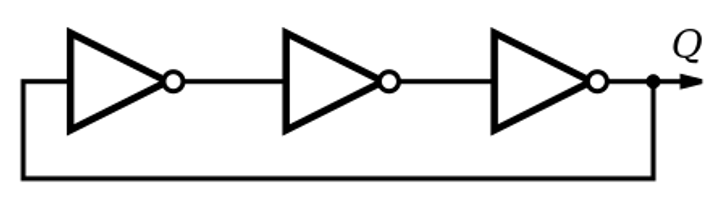
\includegraphics[width = 0.5\textwidth]{img/RingOsc.png}
\end{figure}
\subsubsection{Vnitřní krystalový oscilátor s vnějším rezonátorem}
Aplikace, pro, které je krystalový rezonátor zbytečný, ale RC oscilátor už nevyhoví. Zesilovač nutný pro vznik oscilací je integrován uvnitř mikrokontroléru, ale frekvenčně určující součástky (krystal nebo keramický rezonátor, a k nim případně kondenzátory a rezistory) se připojují zvenčí na piny čipu.

\subsection{Parametry zdrojů hodinových impulsů}
\begin{itemize}
    \item Jmenovitý (nominální) kmitočet
    \begin{itemize}
        \item Jedná se o kmitočet, který je výslovně uveden přímo na pouzdře krystalu.
        \item Krystal je už při samotné výrobě určen pro práci buď na sériovém, nebo na paralelním rezonančním kmitočtu, což se vždy uvádí v katalogovém listu.
        \item Pokud je krystal zkonstruován pro práci na vyšší harmonické frekvenci, je na pouzdře uvedena hodnota této vyšší harmonické.
    \end{itemize}
    \item Tolerance kmitočtu
    \begin{itemize}
        \item Tento parametr udává maximální odchylku reálného kmitočtu od jmenovitého (nominálního) kmitočtu při referenční teplotě 25 °C.
        \item Typické hodnoty tolerance se pohybují v úrovních ±10 ppm, ±20 ppm, ±50 ppm a ±100 ppm (ppm - parts per milion).
    \end{itemize}
    \item Stabilita kmitočtu
    \begin{itemize}
        \item Stabilita definuje maximální odchylku kmitočtu od referenční hodnoty (změřené při 25 °C) v celém rozsahu pracovních teplot daného zařízení.
        \item Podobně jako u tolerance, typické hodnoty jsou ±20 ppm, ±50 ppm a ±100 ppm v celém teplotním rozsahu (což může být například od -40 °C do 85 °C).
    \end{itemize}
    \item Stárnutí (Aging)
    \item \begin{itemize}
        \item Stárnutí popisuje přirozenou změnu rezonančního kmitočtu krystalu v průběhu času.
        \item Změna mechanického namáhání: Po pevněm připájení na desku plošného spoje je krystal mechanicky pnut, postupem času se toto namáhání zmenšuje, což mění frekvenci.
        \item Kontaminace: Během času mohou mikroskopické nečistoty z povrchu krystalu odpadnout, nebo na něj naopak dopadnout, což změní jeho hmotnost a rezonanční kmitočet.
        \item Buzení: Nižší budicí výkon efekt stárnutí zpomaluje. Naopak přebuzení krystalu může stárnutí extrémně urychlit (např. 1 měsíc přebuzení rovná se 1 roku stárnutí).
        \item Efekt stárnutí se s postupujícím časem snižuje. Nejvíce krystal "stárne" během úplně prvního roku svého provozu (typicky pod 5 ppm/rok).
    \end{itemize}
    \item Výkonové zatížení (Drive Level)
    \item \begin{itemize}
        \item Je to maximální výkon, který se smí v krystalu přeměnit v teplo a rozptýlit, aniž by došlo k jeho poškození nebo posunu kmitočtu.
        \item Běžné hodnoty jsou 5 µW pro nízké kmitočty pod 100 kHz a zhruba 1 mW pro kmitočty 1 až 30 MHz. Krystaly pracující na vyšších harmonických snesou 1 až 2 mW.
    \end{itemize}
\end{itemize}

\subsection{Fázový závěs}
Krystalové a keramické rezonátory mají fyzikálně omezený maximální kmitočet. Z hlediska elektromagnetické kompatibility (EMC) je mnohem vhodnější mít na desce vnější oscilátor o nízkém kmitočtu, který tolik nevyzařuje. Zároveň ale samotný procesor a jeho periferie vyžadují pro svůj výpočetní výkon kmitočet vysoký.
Fázový závěs umožňuje násobit (a obecně i dělit) vstupní kmitočet racionálním číslem. Výstupní frekvence je dána vztahem $f_2 = \frac{N}{M} f_1$
\begin{figure}[h!]
    \centering
    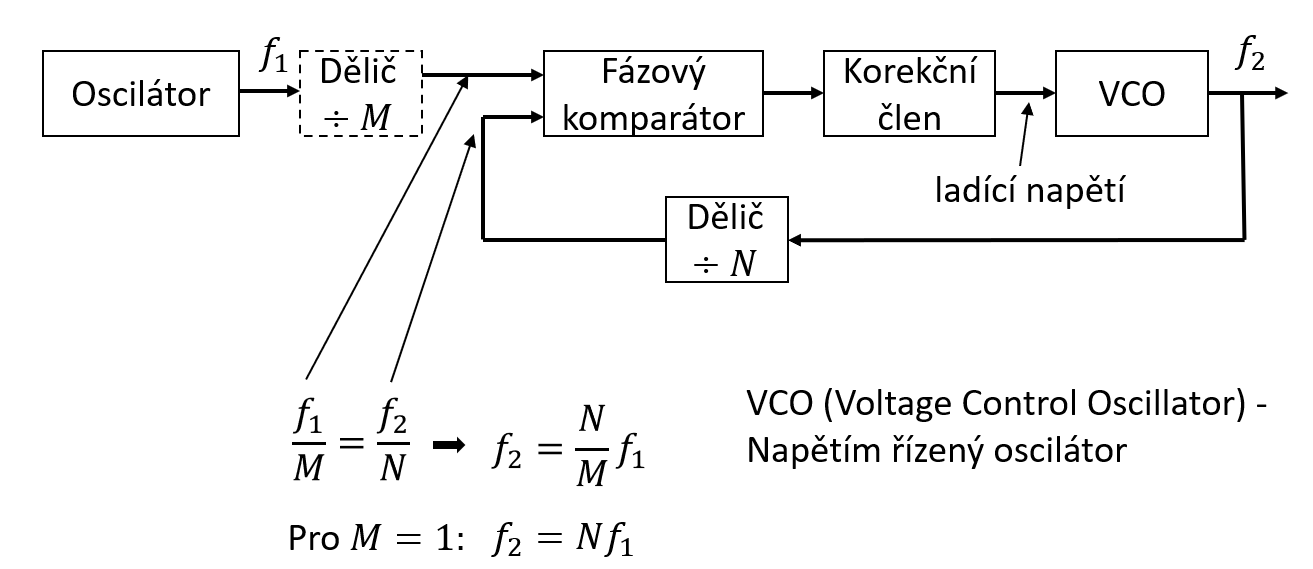
\includegraphics[width =\textwidth]{img/PLL.png}
\end{figure}

\subsection{Watchdog}
\subsubsection{Účel a princip činnosti}
Jeho hlavním úkolem je hlídat, aby procesor neuvízl v nekonečné smyčce nebo „nezabloudil“ (tzv. runaway code).K takovému chybovému stavu může dojít buď chybou v softwaru, nebo hardwarovým problémem (například když rušení nechtěně přepíše obsah paměti).
Hardwarovým základem je čítač, který odpočítává. Pokud tento čítač dosáhne hodnoty 0, automaticky vyvolá RESET celého mikrokontroléru.
\subsubsection{Pasivace (tzv. „krmení psa“)}
Aby k resetu nedošlo, musí běžící program pravidelně tento čítač nastavovat zpět na jeho výchozí hodnotu ještě předtím, než stihne dosáhnout nuly. Toto „krmení psa“ (pasivace) se obvykle provádí zápisem libovolné hodnoty nebo definované sekvence hodnot do příslušného registru.
Zápis pro pasivaci psa nemá absolutně smysl provádět uvnitř přerušovací rutiny. (Důvodem je to, že i když hlavní program zamrzne, časovač přerušení může stále běžet, psa dál krmit, a zařízení by se nikdy neresetovalo).

\subsection{UART(Universal Asynchronous Receiver-Transmitter)}
Jde o asynchronní sériovou komunikaci. To znamená, že hodinový signál se nepřenáší mezi přijímačem a vysílačem; obě komunikující strany musí mít svůj vlastní, nezávislý zdroj hodin.Využívá pouze tři vodiče: Tx (vysílaná data), Rx (přijímaná data) a společnou zem GND .
\begin{figure}[h!]
    \centering
    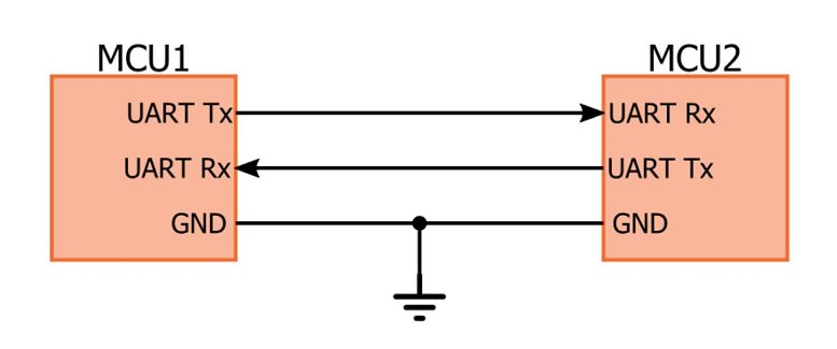
\includegraphics[width =\textwidth]{img/UART.png}
\end{figure}

Komunikace je plně duplexní, tj. data lze odesílat i přijímat současně. Přenosové rychlosti se udávají v baudech (Bd - počet bitů za sekundu), přičemž velmi často používaná hodnota je 9600 Bd. Datový rámec se skládá se ze Start bitu, 8 datových bitů, volitelného paritního bitu (sloužícího k detekci poškození jednoho bitu) a Stop bitu .
\begin{figure}[h!]
    \centering
    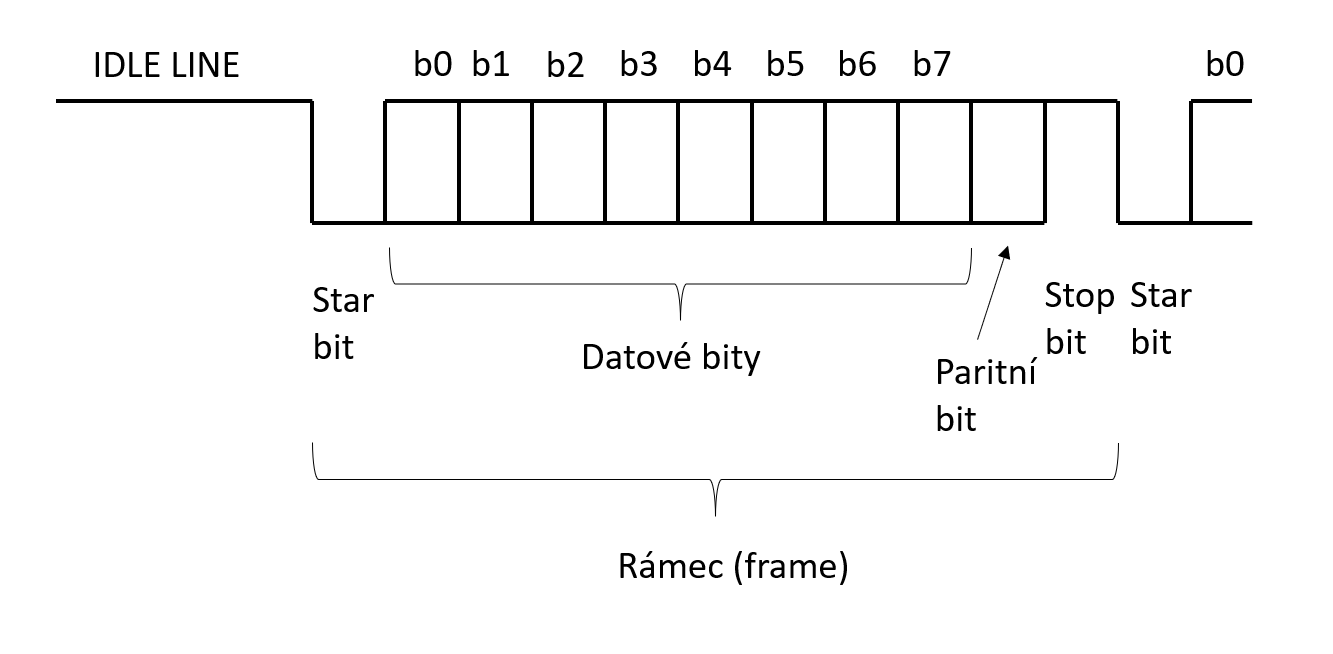
\includegraphics[width =\textwidth]{img/UARTframe.png}
\end{figure}

\subsection{SPI(Serial Peripheral Interface)}
Jde o synchronní komunikaci plně řízenou z pozice Master zařízení.Základem jsou posuvné registry v Masteru i ve Slave.
S každým hodinovým taktem se vysunuje bit z jednoho zařízení a nasouvá do druhého. Během 8 taktů tak dojde ke kompletní vzájemné výměně bajtů mezi Masterem a vybraným Slavem .
\begin{figure}[h!]
    \centering
    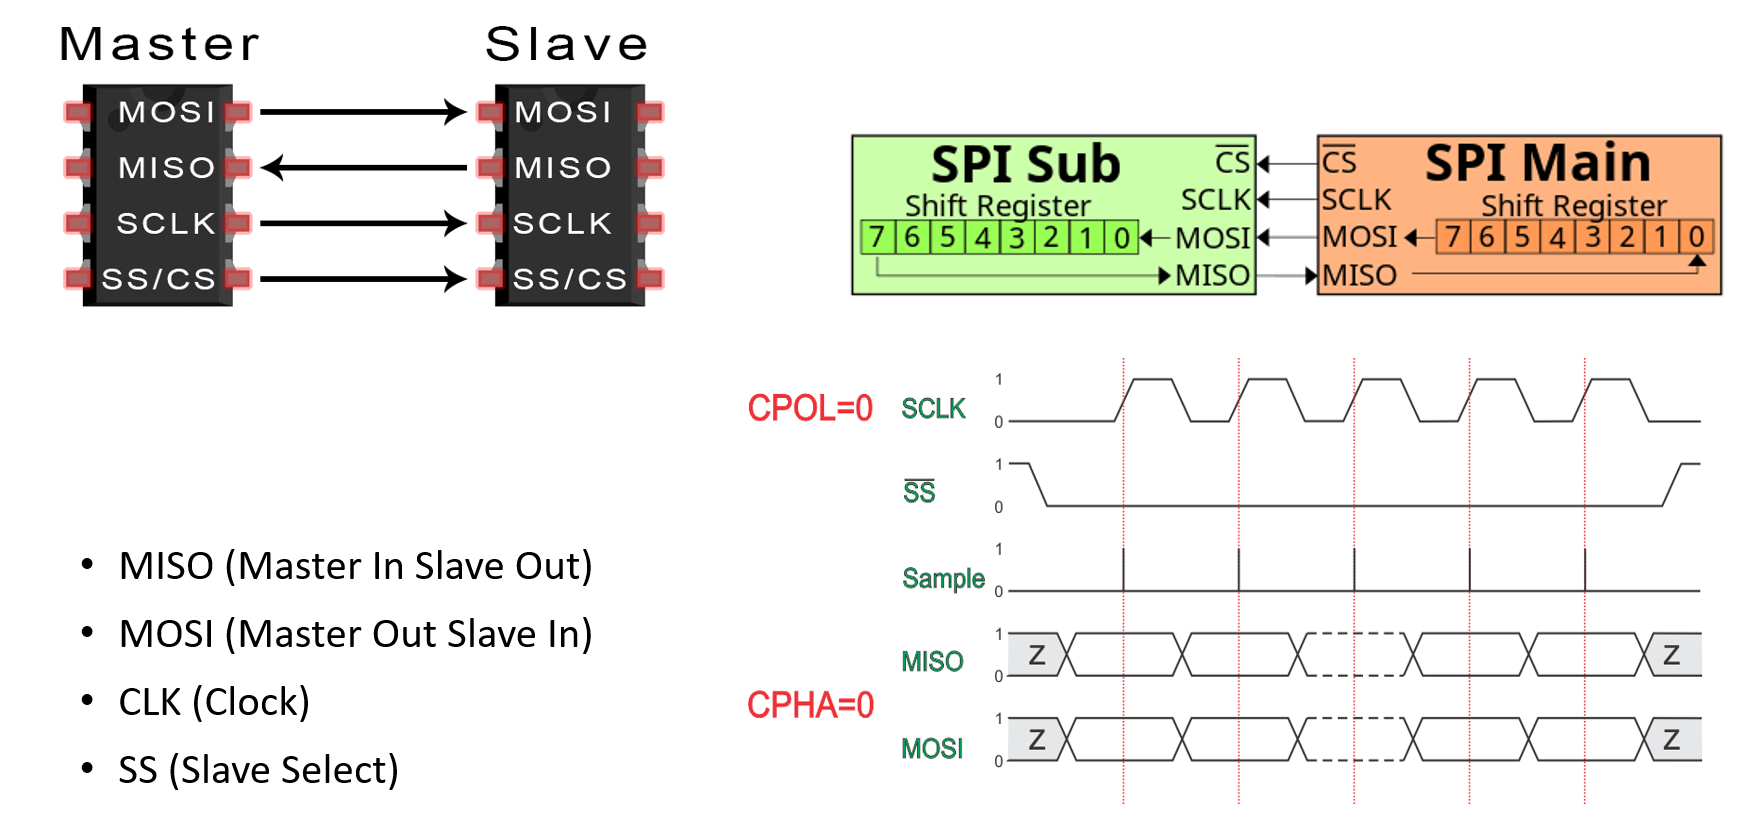
\includegraphics[width =\textwidth]{img/SPI.png}
\end{figure}
Připojení více Slave zařízení: Master vybírá konkrétního Slave tak, že mu aktivuje úroveň na lince SS. Ostatní zařízení s neaktivní úrovní SS musí sběrnici ignorovat.
\begin{figure}[h!]
    \centering
    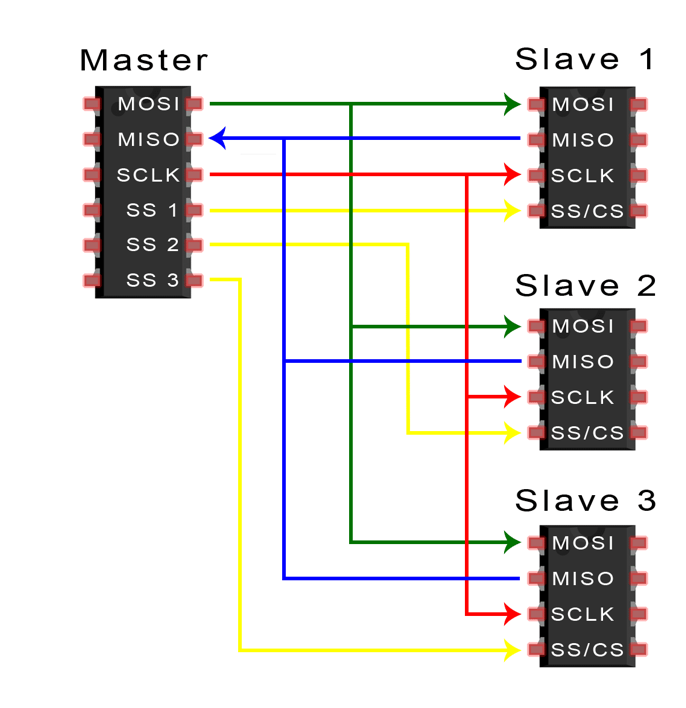
\includegraphics[width =0.5\textwidth]{img/SPImulti.png}
\end{figure}

\FloatBarrier
\subsection{I2C / IIC (Inter-Integrated Circuit)}
Synchronní sériová sběrnice původně vyvinutá firmou Philips pro komunikaci mezi čipy na jedné desce. Vystačí si pouze se 2 signálovými vodiči: SDA (data) a SCL (hodiny generované Masterem).
\begin{figure}[h!]
    \centering
    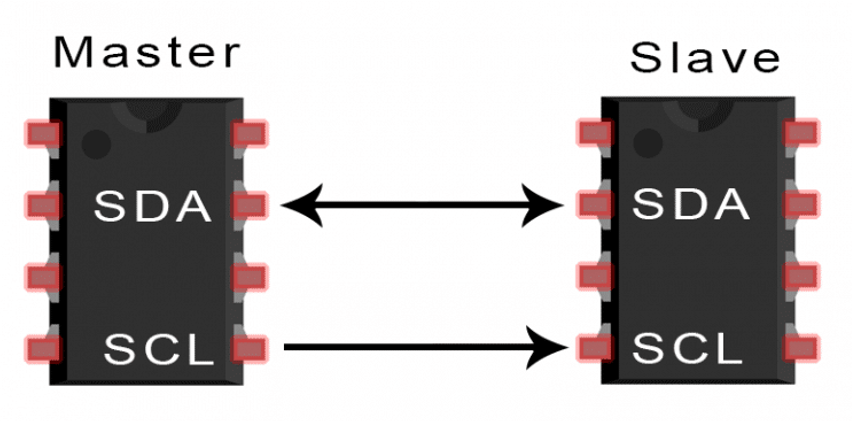
\includegraphics[width =0.5\textwidth]{img/I2C.png}
\end{figure}
Výstupy zařízení musí být zapojeny jako "otevřený kolektor" (Open Drain) a sběrnice musí být vytažena k napájení přes pull-up rezistory. Nízká úroveň (0V) je tzv. dominantní (kterékoliv zařízení může stáhnout sběrnici dolů) a vysoká úroveň je recesivní (pokud nikdo nevysílá nulu, rezistory stáhnou sběrnici nahoru) .
\begin{figure}[h!]
    \centering
    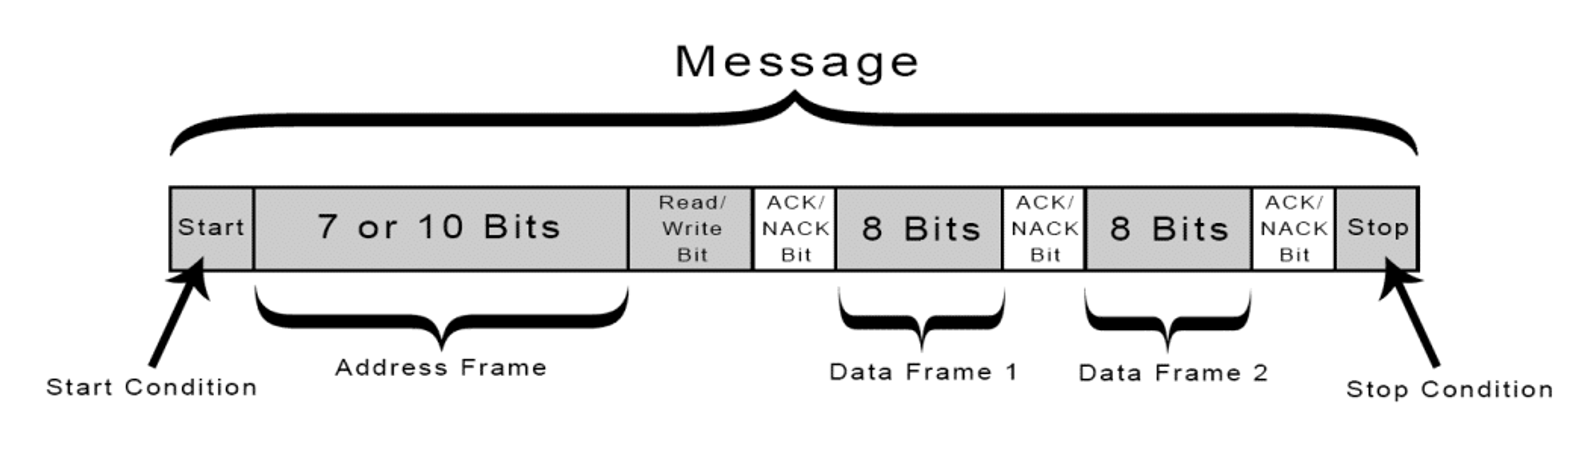
\includegraphics[width =\textwidth]{img/I2Cframe.png}
\end{figure}
Každá transakce začíná tzv. Start condition (SDA padá dolů zatímco SCL drží vysoko) generovanou Masterem.

Sběrnice využívá adresní rámec - každý Slave má svou unikátní 7 nebo 10bitovou adresu. První odeslaný bajt obsahuje tuto adresu a bit určující, zda bude Master následně data číst, nebo zapisovat.

Po odeslání adresního rámce následuje samotný přenos dat, který probíhá vždy v blocích o délce 8 bitů (1 bajt).

Každý bajt na sběrnici musí příjemce potvrdit pomocí bitu ACK (Acknowledge) přidržením vodiče SDA na nízké úrovni.

Aby zařízení Master ukončil probíhající komunikaci a uvolnil sběrnici, musí vygenerovat tzv. Stop condition.
\begin{figure}[h!]
    \centering
    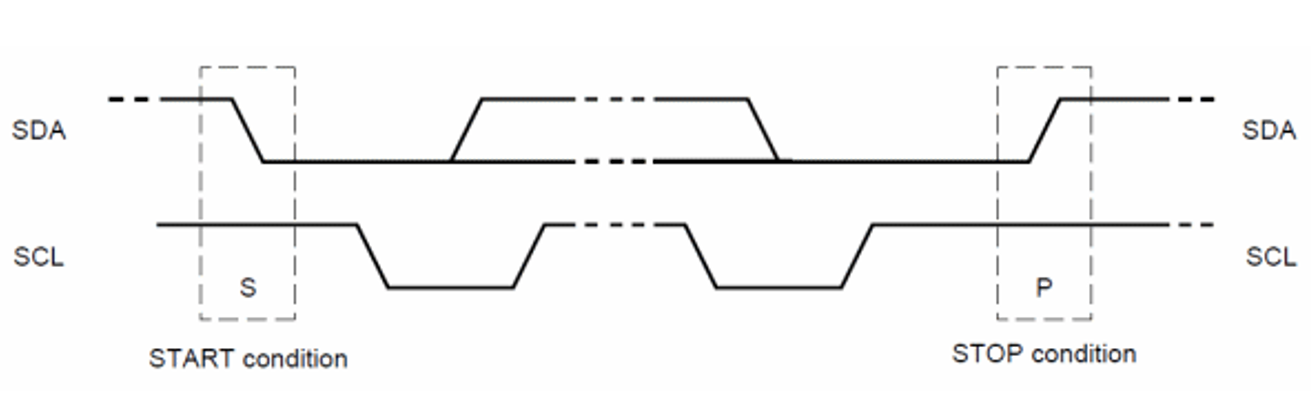
\includegraphics[width =\textwidth]{img/I2Ccond.png}
\end{figure}

Existuje i speciální případ. Pokud chce Master okamžitě vyslat další zprávu (např. po odeslání adresy chce hned číst data) a nechce přitom uvolnit sběrnici (aby mu ji "neukradl" jiný Master), Stop condition vůbec nevyšle. Místo toho rovnou vygeneruje novou Start condition na sběrnici.


